\section{Etapa de búsqueda}
En esta etapa se realiza la búsqueda de instrucciones desde una memoria de 32 bits de ancho de palabra con 128 entradas, siendo entonces de 512 bytes. Usando el  \ac{pc} obtiene la instruccion y la saca hacia un latch para pasar a la etapa de ejecución. \cite{bib:Coad}

\subsection{Introducción}
La etapa de b\'usqueda de instrucci\'on tiene como entradas:
\begin{itemize}
  \item \textbf{rst}: Vuelve a todos los registros a los valores iniciales. 
  \item \textbf{enbl}: Habilita la etapa.
  \item \textbf{dec}: Entrada para la eleccion del contador del programa por si hay algun salto.
  \item \textbf{clk}: Clock de entrada a la etapa.
  \item \textbf{pc\_mux}: Bus que cuenta con el valor del contador de programa que se va a utilizar por si hay un salto.
\end{itemize} 

La etapa tiene como salidas:
\begin{itemize}
	\item \textbf{DR}: Son las instrucciones que entrega la memoria de acuerdo a la entrada que le brinda el \ac{pc}. 
	\item \textbf{pc\_out}: Esta es la salida del \ac{pc} que se traslada a la etapa de decodificación por si hay una instrucción de salto. 
\end{itemize} 

\begin{figure}[H]
\centering
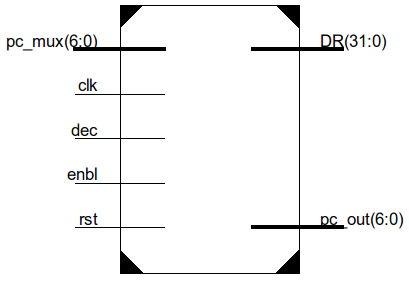
\includegraphics[scale=0.35]{Capitulo01/fetchstage}
\caption{Etapa de búsqueda}
\label{fig:fetch}
\end{figure}

\subsection{Funcionamiento}
El \ac{pc} comienza de 0 y este valor entra en la memoria de instrucciones y en un m\'odulo sumador. En la memoria, para que utilice la instrucci\'on ubicada en la posici\'on del mismo valor de contador de programa, en la entrada del m\'odulo sumador se aumenta en 1 el valor para poder avanzar en el pr\'oximo ciclo de clock a una nueva instrucci\'on. Las salidas de esta etapa son la instrucci\'on a ejecutar y el valor del contador de programa.  (ver Figura \ref{fig:fetchzoom})

\begin{figure}[H]
\centering
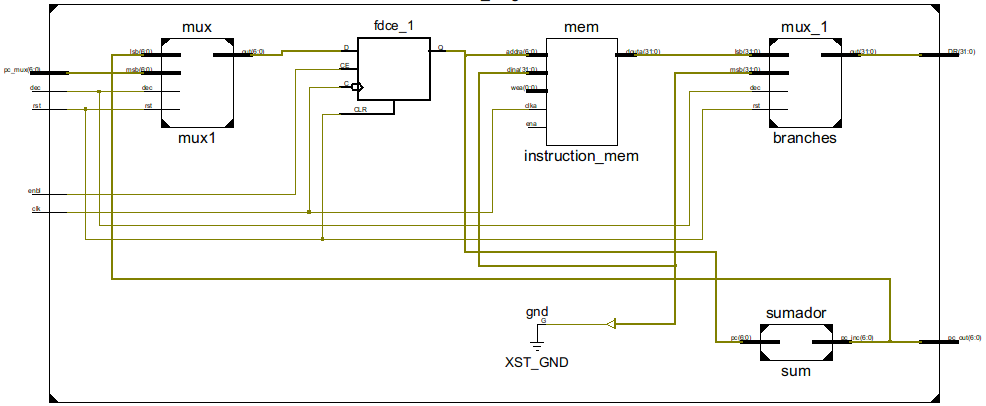
\includegraphics[scale=0.35]{Capitulo01/etapafetchzoom}
\caption{Etapa de búsqueda}
\label{fig:fetchzoom}
\end{figure}

\subsection{Multiplexor}

El módulo multiplexor es binario, osea que solamente elige entre dos valores. En nuestro caso debe escoger entre el \ac{pc} que viene incrementado desde el m\'odulo sumador o el que viene modificado por un salto desde la etapa de ejecución, ver código \ref{mux}. 

\begin{figure}[H]
\centering
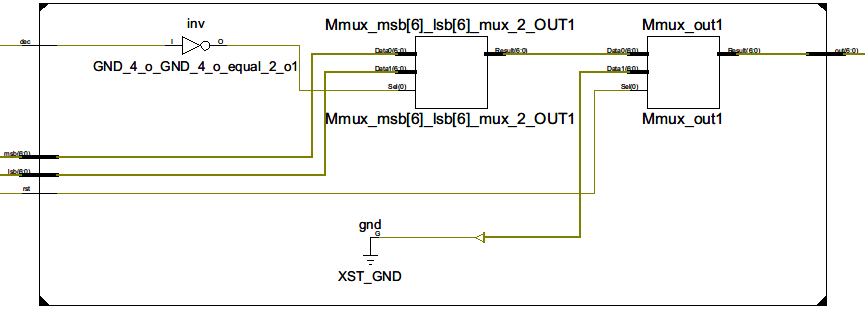
\includegraphics[scale=0.4]{Capitulo01/mux_fig.png}
\caption{M\'odulo multiplexor}
\label{fig:muxmodule}
\end{figure}

En la entrada del multiplexor entran 12 cables para que elija entre la parte alta y la parte baja, dependiendo de si es 1 o 0. Como lo programamos cuando \texttt{dec} est\'a en uno elige el \ac{pc}  que viene incrementado en el otro caso elige el que esta modificado por la etapa de ejecución.

\begin{figure}[H]
\centering
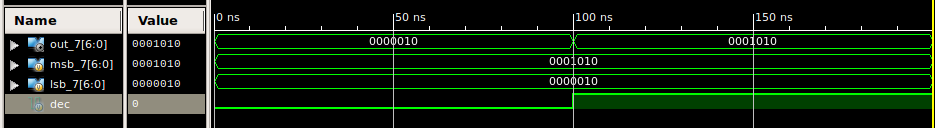
\includegraphics[scale=0.4]{Capitulo01/mux_test}
\caption{Testbench del multiplexor}
\label{fig:muxt}
\end{figure}

El c\'odigo del testbench se puede ver en el apéndice \ref{mux_test} donde se modifica el valor de \texttt{dec} y en los cambios que ocurren se reflejan en la figura \ref{fig:muxt}, en un primer momento \texttt{dec=0} entonces la salida nos da \texttt{0000010} al cambiar el valor pasa a \texttt{0001010}.

\subsection{Incremento}
El m\'odulo sumador simplemente incrementa el \texttt{pc}, el código se muestra en el apéndice \ref{sum}  tiene solamente una entrada que es un bus de 7 bits y este valor es incrementado dentro del m\'odulo. 


\begin{figure}[H]
\centering
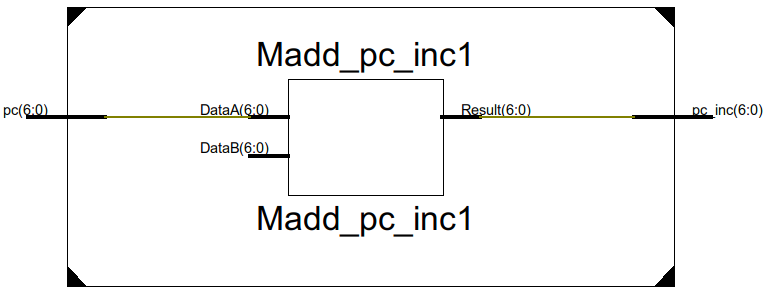
\includegraphics[scale=0.45]{img/sumador_inside}
\caption{Modulo sumador}
\label{fig:sumador}
\end{figure}


En el testbench contador de programa se va modificando de a uno, entonces la salida que en este caso es \texttt{pc\_inc} y esta ingresa en el registro del \texttt{PC}. 


\begin{figure}[H]
\centering
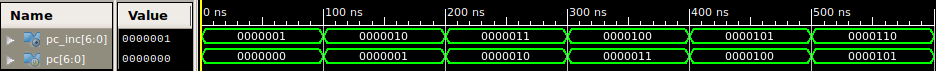
\includegraphics[scale=0.45]{Capitulo01/sum_test}
\caption{Testbench del sumador}
\label{fig:sumt}
\end{figure}


\subsection{Etapa de búsqueda con módulos integrados}
Finalmente generamos un m\'odulo que integre los módulos anteriores generados y terminamos la etapa. El código de la etapa de búsqueda completo se puede ver en el apéndice \ref{fetch}. En este clock solamente el registro \texttt{pc} cambiaría de valor. 

\begin{figure}[H]
\centering
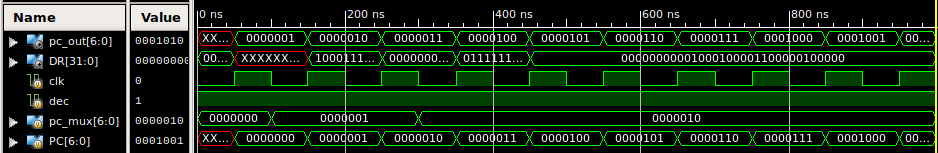
\includegraphics[scale=0.45]{Capitulo01/fetch_test}
\caption{Testbench del modulo fetch}
\label{fig:fetcht}
\end{figure}

Para entender que hace esta etapa podemos ver los cambios en la figura \ref{fig:fetcht}, debemos comenzar viendo que \texttt{PC} no tiene ningún valor y es el que le ingresara en el clock a la memoria de instrucciones, \texttt{pc\_out} tampoco contiene ningún valor y este entra en el multiplexor, la memoria de instrucciones se puede ver en \ref{a.coe}.  
En el primer clock ascendente como \texttt{dec} esta en uno, elige \texttt{pc\_mux} para escribir al \texttt{pc} todos ceros o sea la primera direccion de memoria. El \ac{dr}  muestra  solo x porque en el clock anterior el \ac{pc} estaba en x y en la memoria no direcciona en ninguna posición valida. En el próximo clock ascendente ya el \ac{pc} contiene ceros por lo que automáticamente \texttt{pc\_out} va a tener el valor de \texttt{PC} + 1, pero \texttt{dec} esta en 1 por lo que sigue eligiendo a \texttt{pc\_mux} que en el clock descendente anterior ya se le había aumentado el valor en 1 por lo que este valor va a ser ingresado en el próximo clock al \texttt{pc} y \ac{dr} ya comienza a mostrar el primer valor de la memoria de instrucciones. Los siguientes clocks funcionan de la misma manera.

\lstinputlisting[label=a.coe, caption=Contenido de la memoria de instrucciones, captionpos=b]{Capitulo01/a.coe}